\section{Hudson oraz Jenkins - klasyczne narzędzia do CI/CD}
% tutaj mógłbym zamieścić trochę informacji historycznych jak język java zrewolucjonował inżynierię oprogramowania i dalej rozwinąć, że pokłosiem tego było powstanie Jenkinsa.
% Myślę, że mógłbym tutaj opisać najbardziej uniwersalne rzeczy które są w nim używane. Wydaje mi się że mógłbym poszukać alternatyw do Jenkinsa by rozszerzyć ten dział.
% Jako część tego rozdziału mógłbym zawrzeć problem gdzie konieczne jest użycie Jenkinsa i to byłoby zrobione jako część praktyczna.
% Wbrew pozorom do niektórych zastosować Jenkins nadal jest używany, np do środowisk gdzie QA musi odpalać                    

\subsection{Inżynieria oprogramowania}
Kolejny rozdział tej pracy inżynierskiej poświęcimy na opisanie aspektów automatyzacji w procesach tworzenia oprogramowania. 
Jako wprowadzenie do tego działu kolejny raz chciałbym na podstawie książki "The Phoenix Project: A Novel about IT, DevOps, and Helping Your Business Win" autorstwa Gene Kim i Kevin Behr pokazać jak popularyzacja komputerów spowodowała zapotrzebowanie na nowe technologie. 
Z biegiem czasów gdy komputery stawały się coraz to bardziej popularne, powstawało coraz więcej aplikacji czy to desktopowych czy to webowych. Coraz więcej programistów i aplikacji pojawiało się na rynku. Powstawało wiele firm tworzących oprogramowanie i w związku z dużą konkurencyjnością, firmy wymyślały nowe sposoby poprawy wdrażania oprogramowania, sprawdzania jakości kodu, dostępności infrastruktury oraz poprawy wydajności kodu, po to by wyróżnić się na konkurencyjnym rynku. Coraz to większą rolę w środowisku IT zaczęli odgrywać  DevOpsi, czyli jak podają autorzy książki, osoby tworzące równowagę pomiędzy działami wytwarzania oprogramowania i zarządzania systemami.  


\subsection{DevOps} 
Jak wspomina Gene i Kevin w swojej książce - do głównych zadań inżynierów DevOps należy:
\begin{itemize}
    \item projektowanie strategi kontroli wersji
    \item wdrożenie i integracja kontroli źródeł
    \item implementacja i zarządzanie infrastrukturą build'owania
    \item wdrażanie przepływu kodu
    \item zarządzanie konfiguracją aplikacji i jej tajnymi danymi
\end{itemize}

Autorzy książki opisują duży chaos w zarządzaniu kodem w czasach kiedy wszystkie te koncepty nie były jeszcze tak popularne jak dzisiaj. Opisują środowiska przechowywania kodu jako miejsca mało zadbane i prowadzone bez głębszego pomysłu.

DevOps to podejście do rozwoju oprogramowania, które obejmuje ciągły rozwój, ciągłe testowanie, ciągłą integrację, ciągłe wdrażanie i ciągłe monitorowanie oprogramowania w całym cyklu jego życia. Jest to proces przyjęty przez wszystkie najlepsze firmy w celu opracowania wysokiej jakości oprogramowania i skrócenia czasu tworzenia produktu, co przekłada się na większą satysfakcję klientów, czego każda firma poszukuje.
Inżynierowie DevOps codziennie korzystają z wielu narzędzi jak Kibana czy Splunk do monitorowania aplikacji, Git czy Mercurial do zarządzania kodem, Puppet, Ansible bądź Chef do zarządzania konfiguracją i wiele innych. 
W dalszej części pracy skupimy się na narzędziu, które subiektywnym zdaniem autorów tej pracy najlepiej obrazuje codzienne zadania automatyzujące inżynierów DevOps czyli Jenkins.
Na potwierdzenie słuszności naszego wyboru warto dodać, że narzędzie to w 2011 roku wygrało nagrodę Bossie (Best of Open Source Software Award) oraz w 2014 prestiżową nagrodę Geek Choice.  

\subsection{Projekt}

Celem projektu jest przybliżenie możliwości automatyzacji na podstawie nowoczesnego narzędzia codziennie wykorzystywanego w świecie IT. Tym narzędziem będzie Jenkins. 
Na potrzeby tego projektu stworzę również prostą aplikację Spring Boot, która będzie implementowała podstawowe założenia API RESTful. Jenkins oraz aplikacja w nawiązaniu do poprzedniego działu tej pracy będą uruchomione na kontenerach. Celem tego zabiegu jest zaprezentowanie działania tego narzędzia. 

\subsection{Jenkins}

Jest to projekt open sourcowy (co oznacza, że każdy może wprowadzać zmiany do projektu) napisany całkowicie w języku Java. Jenkins wykonuje szereg zadań by osiągnąć założenia ciągłej integracji poprzez automatyzację części związanych z budowaniem, testowaniem i wdrażaniem. To sprawia, że developerzy mogą ciągle pracować nad ulepszaniem produktu nad którym pracują. Ponadto jest to system, który działa na servletowych kontenerach, jak na przykład Apache Tomcat. 
Jenkins automatyzuje budowanie aplikacji, dzięki czemu developerzy są w stanie wcześnie wykrywać błędy w swoim kodzie. Do głównych zalet Jenkinsa zdecydowanie można zaliczyć społeczność, która się wokół Jenkinsa przez wiele lat działalności zbudowała. Jest to narzędzie nie tylko łatwo rozszerzalne, ale również posiada wiele zaimplementowanych wtyczek. 
Kilka przykładów zastosowania tego oprogramowania:
\begin{itemize}
    \item budowanie aplikacji przy pomocy narzędzi do buildowania jak Gradle, Maven czy inne 
    \item automatyzacja testów  (Nose2, PyTest, Robot, Selenium i wiele innych)
    \item wykorzystywany do testowania skryptów (bash, bat, zsh, inne)
    \item raportowanie, czyli na przykład wyświetlanie wyników testów
\end{itemize}

Na czas pisania tej pracy Jenkins posiada ponad 1500 wtyczek stworzonych przez społeczność, dzięki którym doświadczenie z korzystania z narzędzia oraz aktywności związane z budowaniem, wdrażaniem i automatyzacją projektu stają się lepsze. 

\subsection{Historia}

Jenkins nie zawsze nosił nazwę taką jak dziś. Został stworzony przez pracownika Sun Microsystems Kohsuke Kawaguchi w lato 2004 roku, a pierwsze wydanie nastąpiło w styczniu 2005 roku pod nazwą "Hudson". Oprogramowanie występuje pod nazwą Jenkins od 2011 roku po tym jak firma Sun Microsystems została wykupiona przez firmę Oracle. Na początku Hudson i Jenkins były tworzone osobno, ale po przejęciu firmy zarząd postanowił połączyć oba projekty i zachować nazwę Jenkins, gdyż posiadał on znacząco większą społeczność niż projekt Hudson. Dzisiaj wsparcie dla projektu Hudson nie jest oficjalnie prowadzone. 

\subsection{Architectura}

Aby dobrze zrozumieć jak działa narzędzie, w tym rozdziale opiszę co się stanie jeśli developer zapisze zmiany na repozytorium, przedstawię przykładową implementację metodologii ciągłej integracji/ciągłego wdrażania w Jenkinsie oraz opiszę jak wygląda architektura Master-Slave.

Według Johna Smart, czyli autora książki "Jenkins: The Definitive Guide" istnieje kilka kroków, które opisują jak działa komunikacja między elementami w Jenkinsie: 
\begin{itemize}
    \item inżynier zmienia kod źródłowy aplikacji i zapisuje zmiany do repozytorium
    \item repozytorium jest regularnie sprawdzane przez serwer Jenkins CI i w razie jakiś zmian ten sam serwer pobiera je do dalszej pracy
    \item w następnym kroku jest sprawdzane czy zapisane zmiany "przechodzą". Build  jest wykonywany i jeśli nie było żadnych błędów generowany jest plik wykonywalny. Jeśli pojawią się jakieś błędy, tworzony jest email z linkiem do logów builda. 
    \item w przypadku gdy build był udany, plik wykonywalny jest wdrażany na środowisku testowym. Ten krok pomaga zrealizować krok ciągłego testowania ponieważ plik wykonywalny przechodzi przez wiele testów automatycznych. Jeśli są problemy w którymś z testów, programiści również są o tym informowani.
    \item jeśli nie ma problemów podczas buildu, integracji czy testowania - zmiany są automatycznie wdrażane na środowisko produkcyjne
\end{itemize}



Często się zdarza, że pojedynczy serwer może nie wystarczyć. Na przykład:
\begin{itemize}
    \item testy muszą być wykonane na różnych środowiskach
    \item pojedynczy serwer nie jest wstanie obsłużyć ruchu, który jest wymagany w wielkich systemach.
\end{itemize}

W tych przypadkach wykorzystywana jest architektura Master-slave, wspomniana krótko na początku tego działu. Jak więc wygląda ta architektura? O tym właśnie będzie dalsza część tej pracy. 
Architektura master-slave jest używana do zarządzania rozszerzonymi buildami. Komunikacja między serwerem mastera i slave'a odbywa się poprzez protokół TCP/IP. 

\subsection{Master}

To jest główny serwer Jenkinsa. Do jego głównych zadań należą:
\begin{itemize}
    \item zorganizowanie "jobów" builda
    \item wybór odpowiedniego slave'a
    \item monitorowanie slave'ów i w razie potrzeby włączanie/wyłączanie ich
    \item raportowanie wyników builda do developerów
\end{itemize}

Master również może zostać wykorzystywany bezpośrednio do wykonywania jobów ale rekomendowane jest, żeby były one wykonywane na slaveach.

\subsection{Slave}

Slave'ami nazywami zewnętrzną maszyne połączoną z Masterem. Zależnie od projektu oraz wymagań builda liczna slave'ow może się różnić. Slavy mogą być uruchomione na różnych systemach operacyjnych i zależnie od wymagań builda, master wybiera odpowiedniego slavea do wykonania builda i testów. 
Do głównych zadań slave'a należą:
\begin{itemize}
    \item nasłuchiwanie na polecenia Mastera
    \item wykonie jobów zleconych przez Mastera
    \item developerzy mogą "ręcznie" wybrać slave na którym ma zostać wykonane zadanie ale z reguły Master dobiera najbardziej pasujący slave.
\end{itemize}

\begin{figure}[htbp]
    \centering
    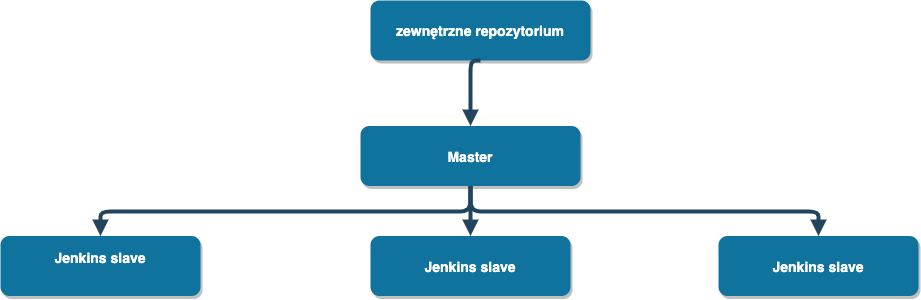
\includegraphics[width=10cm]{master-slave.png}
    \caption{master-slave architektura}
    \label{fig:master-slave}
\end{figure}

Jak do tej pory pokrótce opisaliśmy za co odpowiedzialne są poszczególne komponenty w Jenkinsie. Przedstawię teraz przykładową architekturę oraz opiszę za co są odpowiedzialne poszczególne jej elementy 

\begin{figure}[htbp]
    \centering
    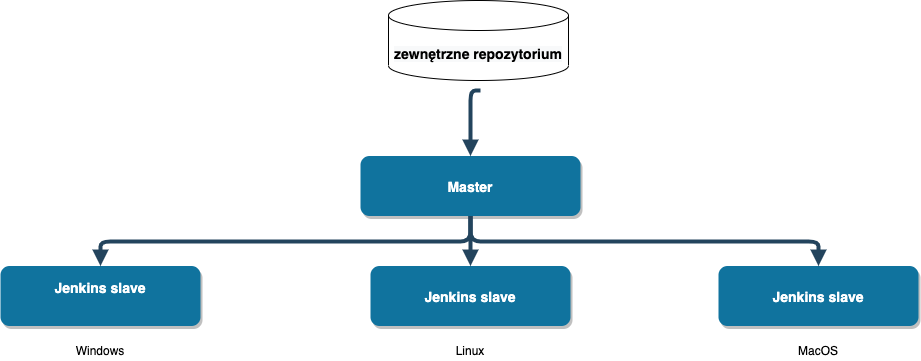
\includegraphics[width=10cm]{archritektura-przyklad.png}
    \caption{architektura przykład}
    \label{fig:jenkins-architektura}
\end{figure}

\begin{itemize}
    \item Developer zapisuje zmiany w kodzie na zewnętrznym repozytorium
    \item master jest połączony z repozytoriom i regularnie sprawdza czy pojawiły się jakieś zmiany. Wszystkie slave'y są połączone z masterem.
    \item master otrzymuje żądanie wykonania zadania, które zostaje przekazane do odpowiedniego slave'a. 
    \item slave wykonuje zlecone zadania, generuje raporty testów. Master ciągle monitoruje wyniki testów.
\end{itemize}

W dalszej części pracy zaprezentujemy przykładowe zastosowanie tego narzędzia. 

\subsection{Aplikacja}

Aplikacja implementuje REST api i będzie wyświetlała imię użytkownika podane do path URL. Projekt posiada proste pliki java w których jest umieszczona logika naszej aplikacji oraz pliki Maven'a do budowania naszej aplikacji. Tak oto wygląda kod pliku pom.xml 

\begin{lstlisting}
    <?xml version="1.0" encoding="UTF-8"?>
<project xmlns="http://maven.apache.org/POM/4.0.0" xmlns:xsi="http://www.w3.org/2001/XMLSchema-instance"
	xsi:schemaLocation="http://maven.apache.org/POM/4.0.0 https://maven.apache.org/xsd/maven-4.0.0.xsd">
	<modelVersion>4.0.0</modelVersion>
	<parent>
		<groupId>org.springframework.boot</groupId>
		<artifactId>spring-boot-starter-parent</artifactId>
		<version>2.3.2.RELEASE</version>
		<relativePath/>
	</parent>
	<groupId>com.example</groupId>
	<artifactId>rest-service</artifactId>
	<version>0.0.1-SNAPSHOT</version>
	<name>rest-service</name>
	<description>Demo project for Spring Boot</description>

	<properties>
		<java.version>1.8</java.version>
	</properties>

	<dependencies>
		<dependency>
			<groupId>org.springframework.boot</groupId>
			<artifactId>spring-boot-starter-web</artifactId>
		</dependency>

		<dependency>
			<groupId>org.springframework.boot</groupId>
			<artifactId>spring-boot-starter-test</artifactId>
			<scope>test</scope>
			<exclusions>
				<exclusion>
					<groupId>org.junit.vintage</groupId>
					<artifactId>junit-vintage-engine</artifactId>
				</exclusion>
			</exclusions>
		</dependency>
	</dependencies>

	<build>
		<plugins>
			<plugin>
				<groupId>org.springframework.boot</groupId>
				<artifactId>spring-boot-maven-plugin</artifactId>
			</plugin>
		</plugins>
	</build>

</project>

\end{lstlisting}

W pliku tym znajdują się zależności jak i wtyczki Spring Boot potrzebne do działania naszej aplikacji. 

\subsection{Dockerfile} 

Dockerfile jest to specyficzny plik, któremy pozwala nam zdefiniować jak powinien nasz kontener wyglądać. Każda linia w Dockerfile to osobna instrukcja, która opisuje jak powinien wyglądać końcowy kontener. 

Na początku konieczne jest zbudowanie naszego programu, żeby można było go wykorzystać w naszym dockerfile. W tym celu użyję komendy ./mvnw clean package, która skompiluje nasz kod i spakuje go do pliku wykonywalnego rest-service-0.0.1-SNAPSHOT.jar. Plik ten będzie wykorzystywany w naszym Dockerfile. 

\begin{lstlisting}
    FROM openjdk:8-jdk-alpine
    VOLUME /tmp
    ADD target/rest-service-0.0.1-SNAPSHOT.jar app.jar
    ENTRYPOINT ["java","-jar","app.jar"]
    EXPOSE 2222
\end{lstlisting}


Każda linia tego pliku dodaje dodatkową funkcjonalność do naszego projektu, więc warto wyjaśnić co w każdej linii się znajduje. W pierwszej linii importujemy dostępny w oficjalnym repozytorium Dockera linuxowy obraz alpine wraz z zainstalowanym na nim openjdk. Alpine Linux jest to podstawowy system operacyjny charakteryzujący się prostotą oraz małym rozmiarem pojemności dyskowej jaką zajmuje. Nie posiada on zbędnych bibliotek, które niepotrzebnie zajmowałyby miejsce na naszym kontenerze, stąd też nasz wybór padł właśnie na ten kontener. Następnie dodajemy wcześniej spakowany plik jar, który znajduje się w folderze /target. Kolejno zaznaczamy jaka komenda powinna zostać uruchomiona po uruchomieniu kontenera oraz udostępniamy port 2222 do dostępu publicznego. 

Kolejno w konsoli użyłem trzech komend, aby zbudować nasz projekt i uruchomić go w kontenerze. 
\begin{lstlisting}
    mvn clean install 
    docker build -t pracainzynierka
    docker run pracainzynierska -p 2222:2222
\end{lstlisting}
W pierwszej kolejności lokalnie budujemy projekt by zaktualizować nasz plik jar, który jest nam potrzebny podczas budownia obrazu Dockera w drugiej komendzie. W ostatnim kroku uruchamiamy nasz kontener. Po tych krokach wchodząc pod adres http://127.0.0.1:2222/greeting otrzymamy powitalną odpowiedź z naszego kontenera. 
W dalszej części pracy inżynierskiej zautomatyzujemy ten proces przy pomocy Jenkinsa. 

\subsection{Automatyzacja przy użyciu Jenkinsa}

Jako, że użyliśmy dockera by uruchomić naszą aplikację lokalnie, nic nie stoi na przeszkodzie by również użyć Dockera do pracy z Jenkinsem. Problemem jaki napotkaliśmy podczas implementacji tego rozwiązania polegał na braku komend dockera wewnątrz kontenera, dlatego trzeba było dodać kilka warstw do naszego Jenkinsowego Dockerfile by umożliwić taką funkcjonalność. 

finalna wersja pliku Dockera wygląda następująco: 

\begin{lstlisting}
    from jenkins/jenkins:lts
    USER root
    RUN apt-get update -qq \
    && apt-get install -qqy apt-transport-https ca-certificates curl gnupg2 software-properties-common
    RUN curl -fsSL https://download.docker.com/linux/debian/gpg | apt-key add -
    RUN add-apt-repository \
   "deb [arch=amd64] https://download.docker.com/linux/debian \
   $(lsb_release -cs) \
   stable"
    RUN apt-get update  -qq \
    && apt-get install docker-ce=17.12.1~ce-0~debian -y
    RUN usermod -aG docker jenkins
\end{lstlisting}

Kolejno przy użyciu dwóch kolejnych komend:
\begin{lstlisting}
    docker image build -t jenkins-docker .
    docker container run -d -p 8080:8080 -v /var/run/docker.sock:/var/run/docker.sock jenkins-docker
\end{lstlisting}

jesteśmy w stanie wchodząc pod adres 127.0.0.1:8080 finalnie dostać się do Jenkinsa

\subsection{Konfigurowanie Jenkinsa}

Głównymi narzędziami, które będzie trzeba skonfigurować jest JDK, Maven oraz GIT, by móc budować aplikacje oraz klonować kod z repozytorium. Wszystkie kroki wykonuje się z poziomu Jenkinsa. W naszym projekcie konfiguracja wygląda jak na zrzutach ekranu poniżej:

\begin{figure}[htbp]
    \centering
    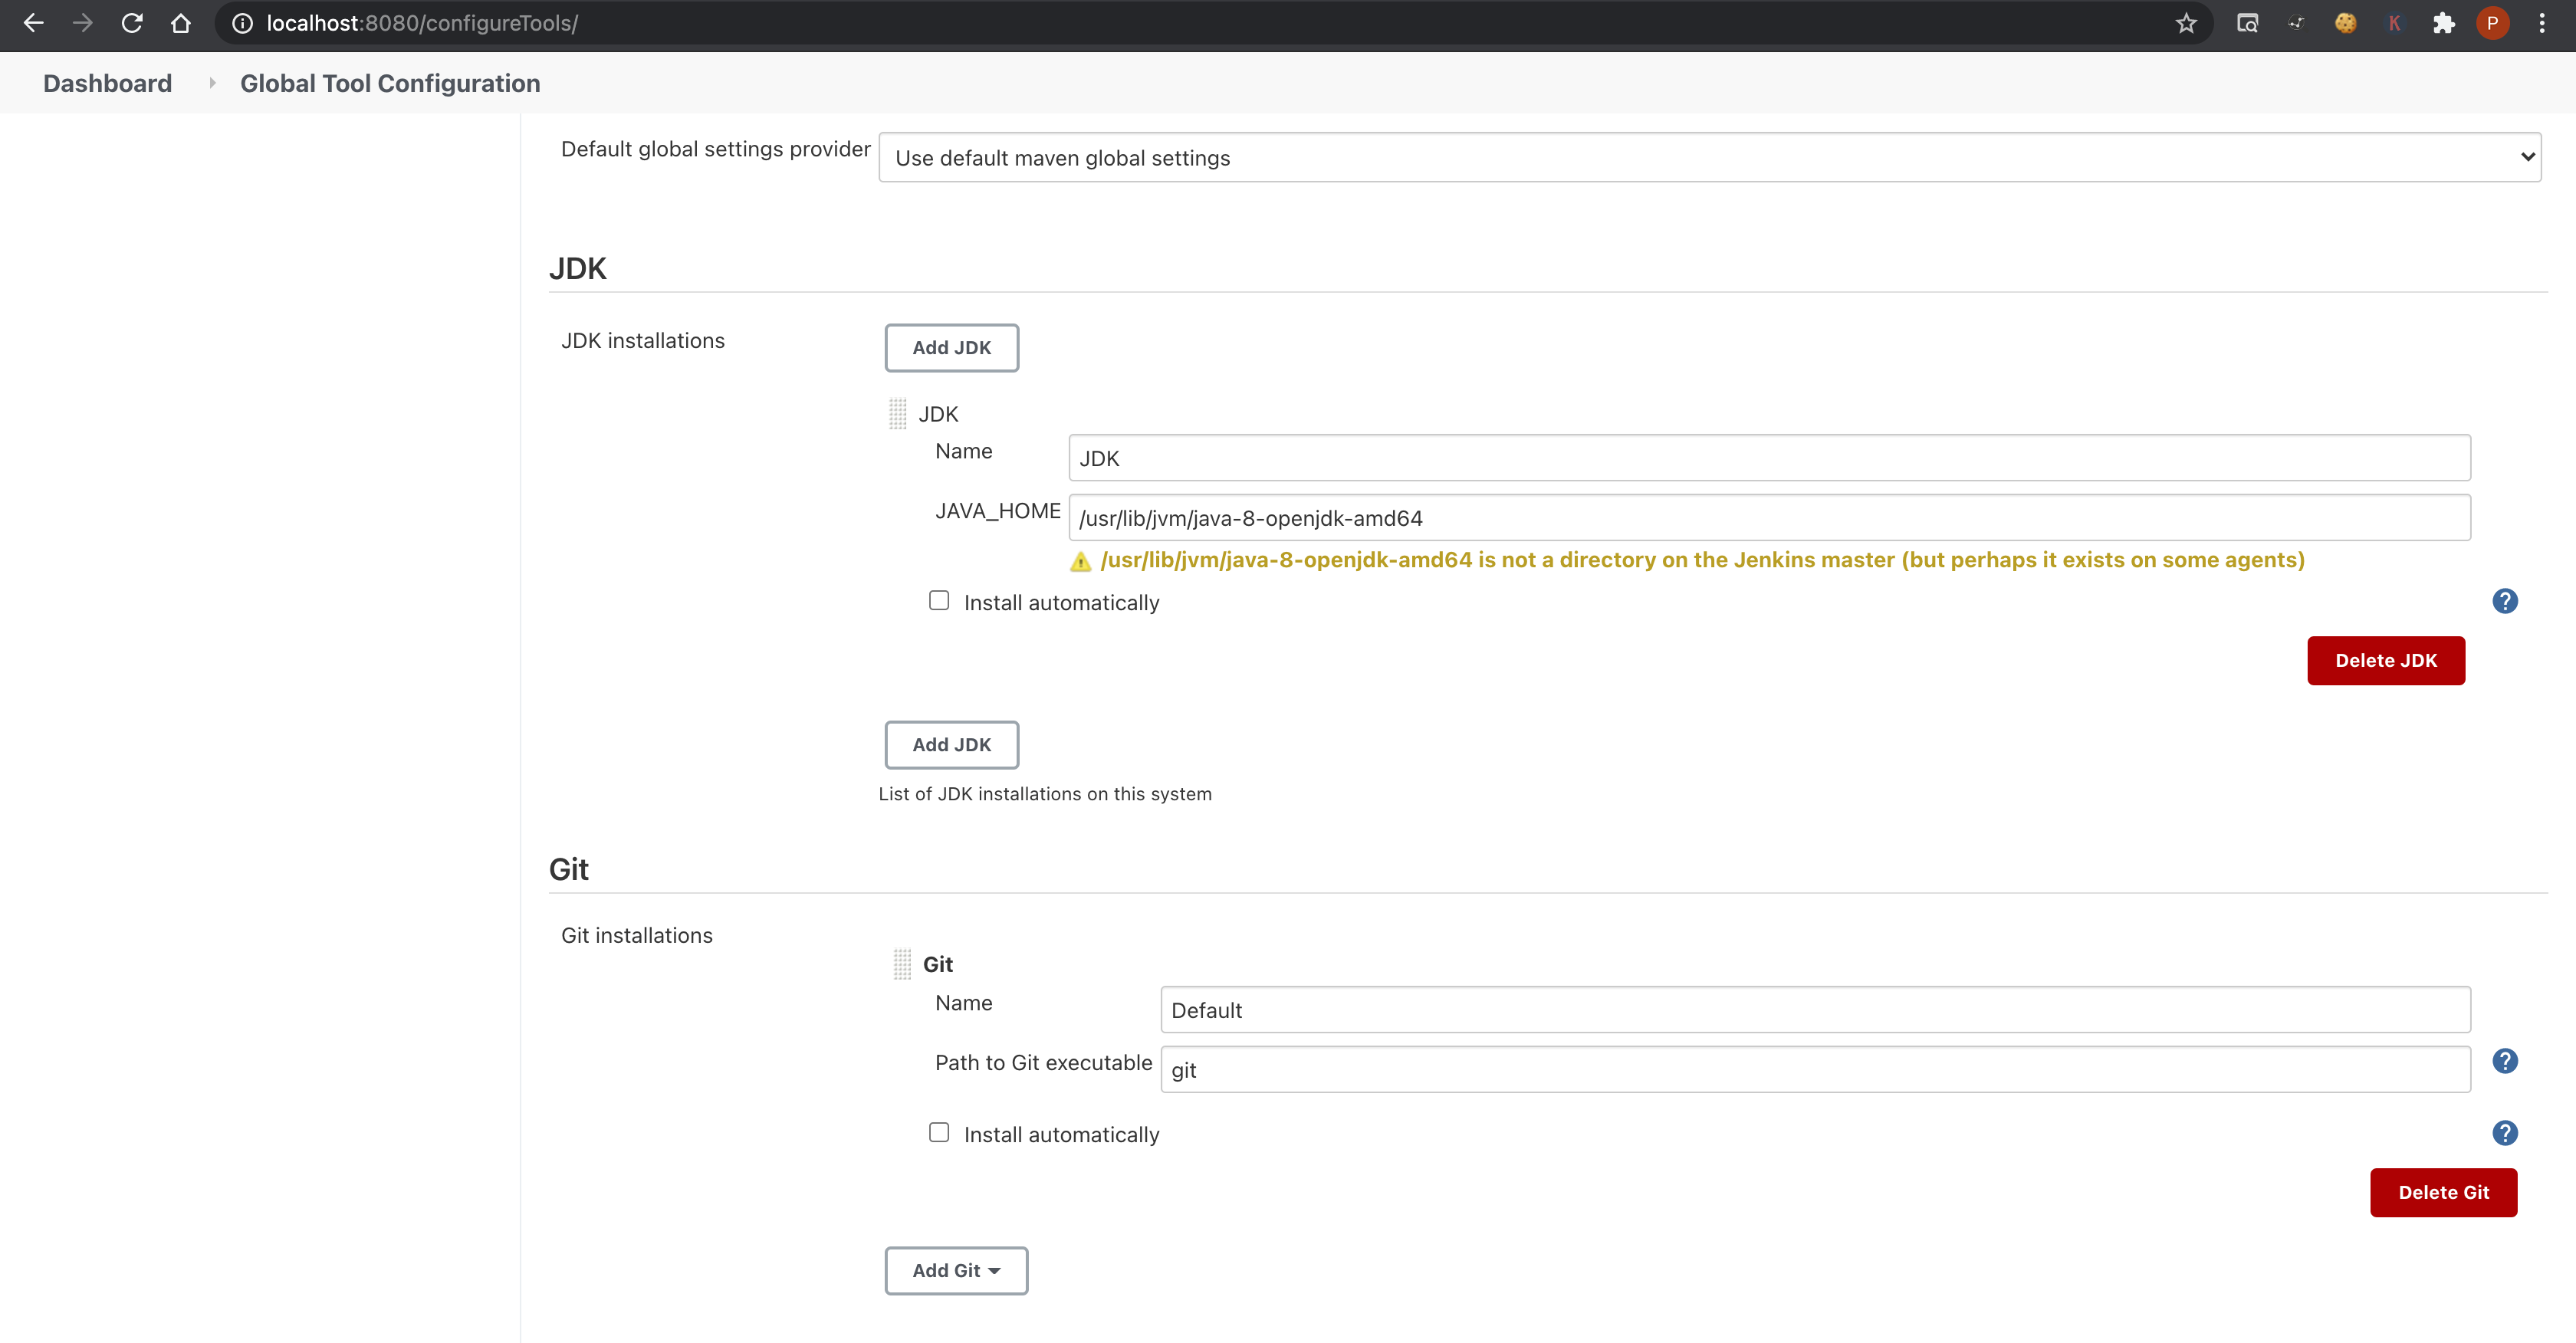
\includegraphics[width=10cm]{iz-JKD-Git.png}
    \caption{JDK-Git}
    \label{fig:JDK-Git}
\end{figure}
\begin{figure}[htbp]
    \centering
    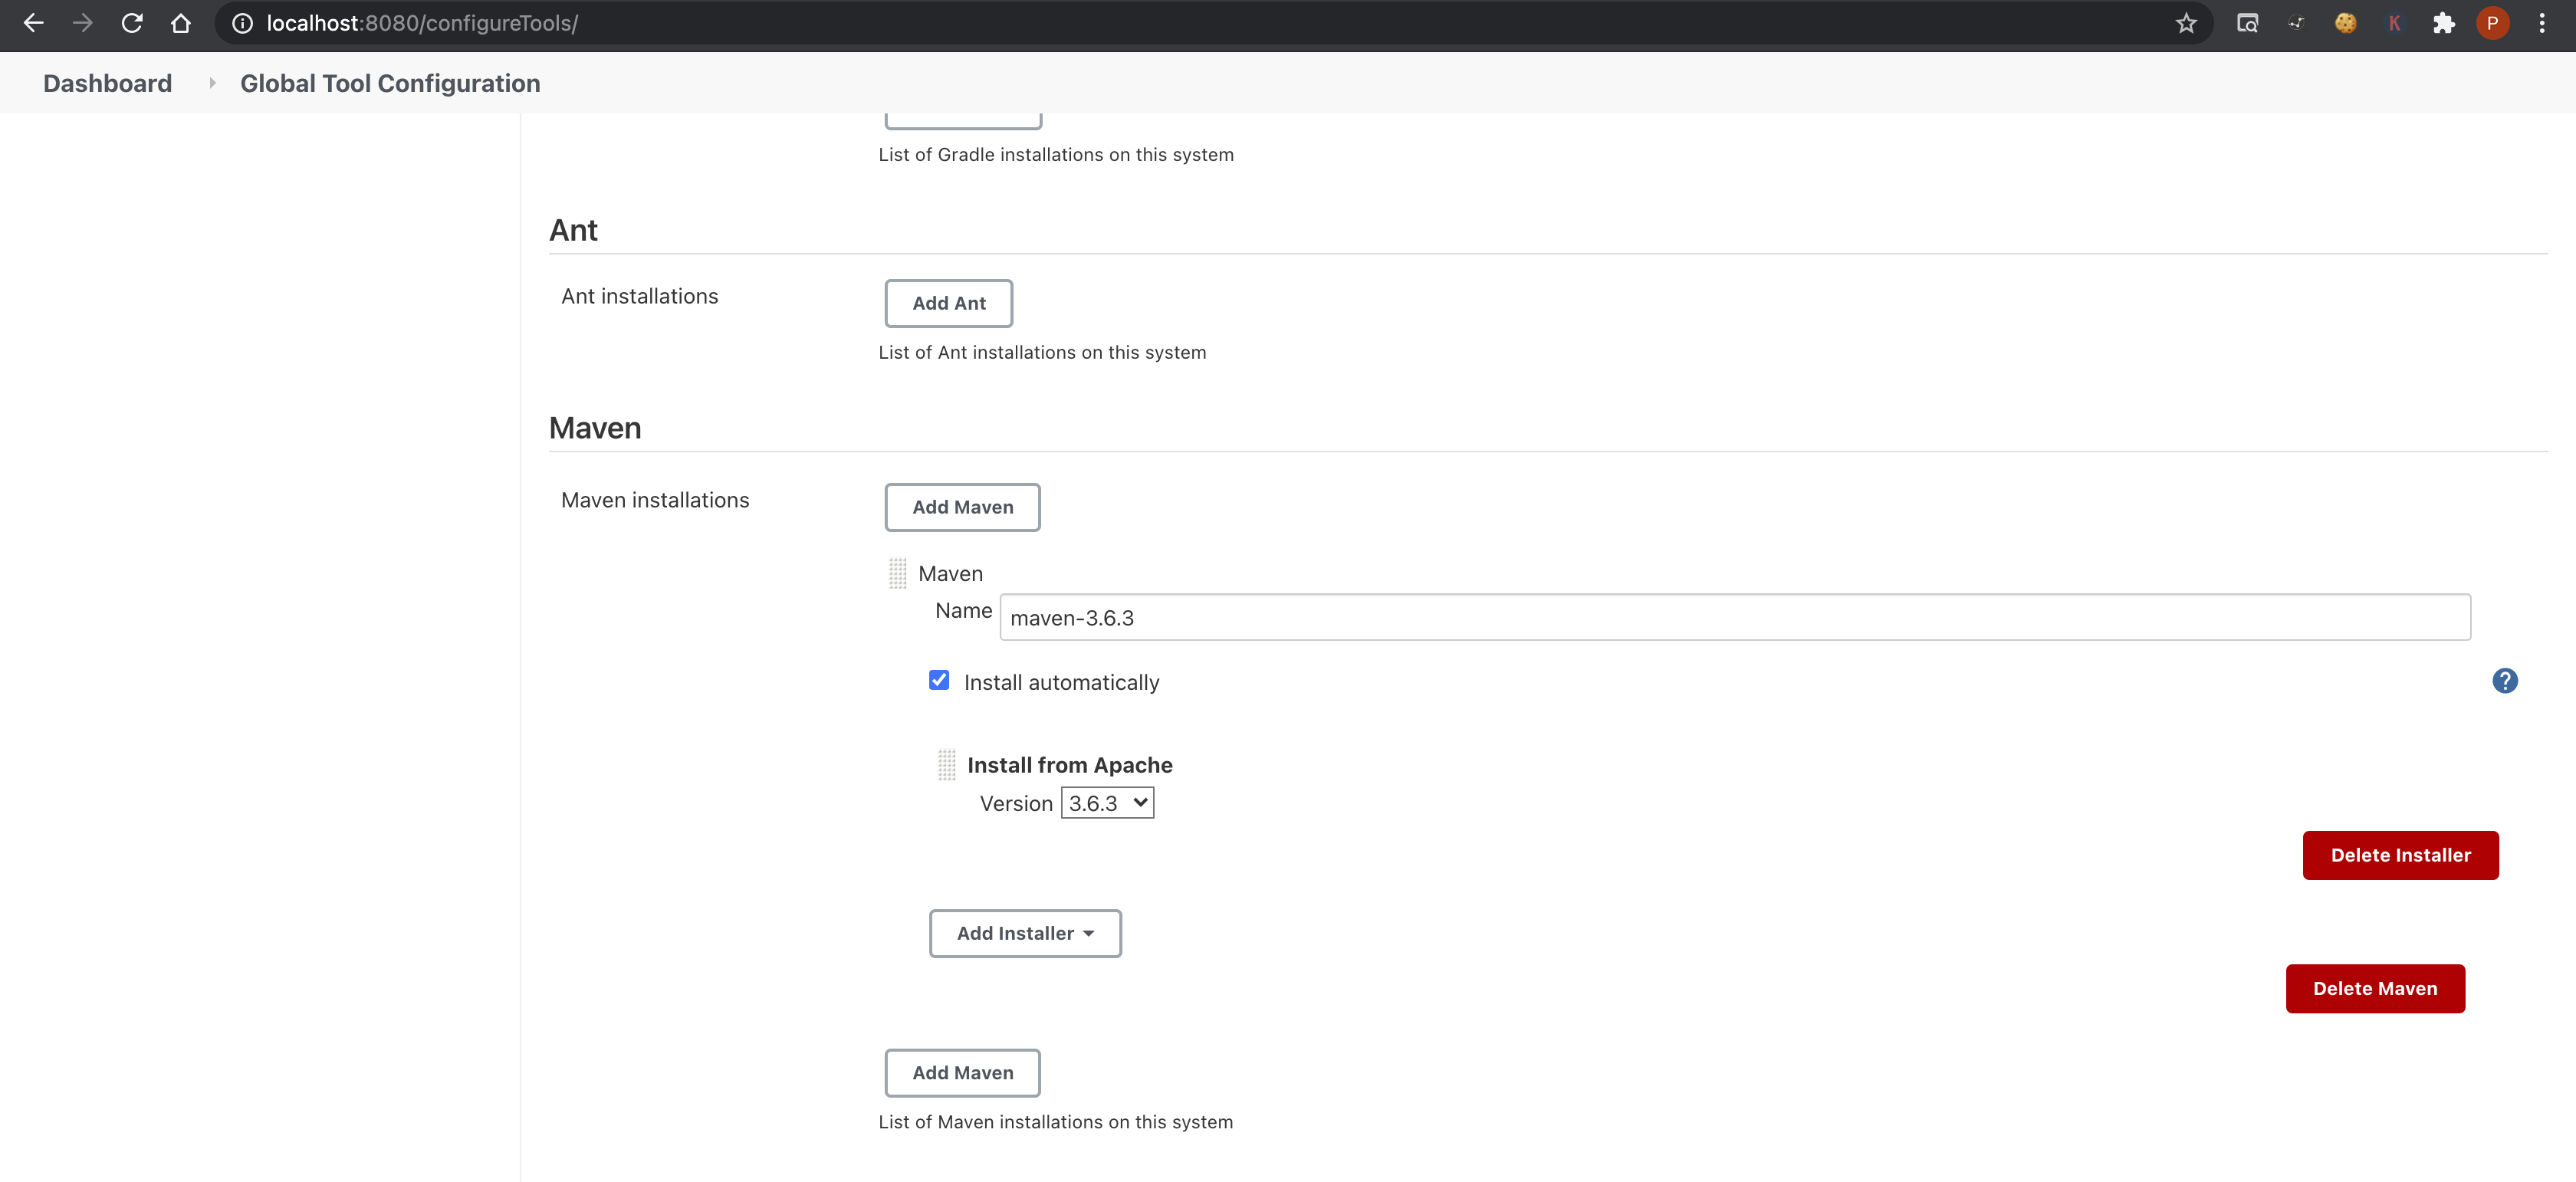
\includegraphics[width=10cm]{iz-maven.png}
    \caption{maven}
    \label{fig:maven}
\end{figure}
\begin{figure}[htbp]
    \centering
    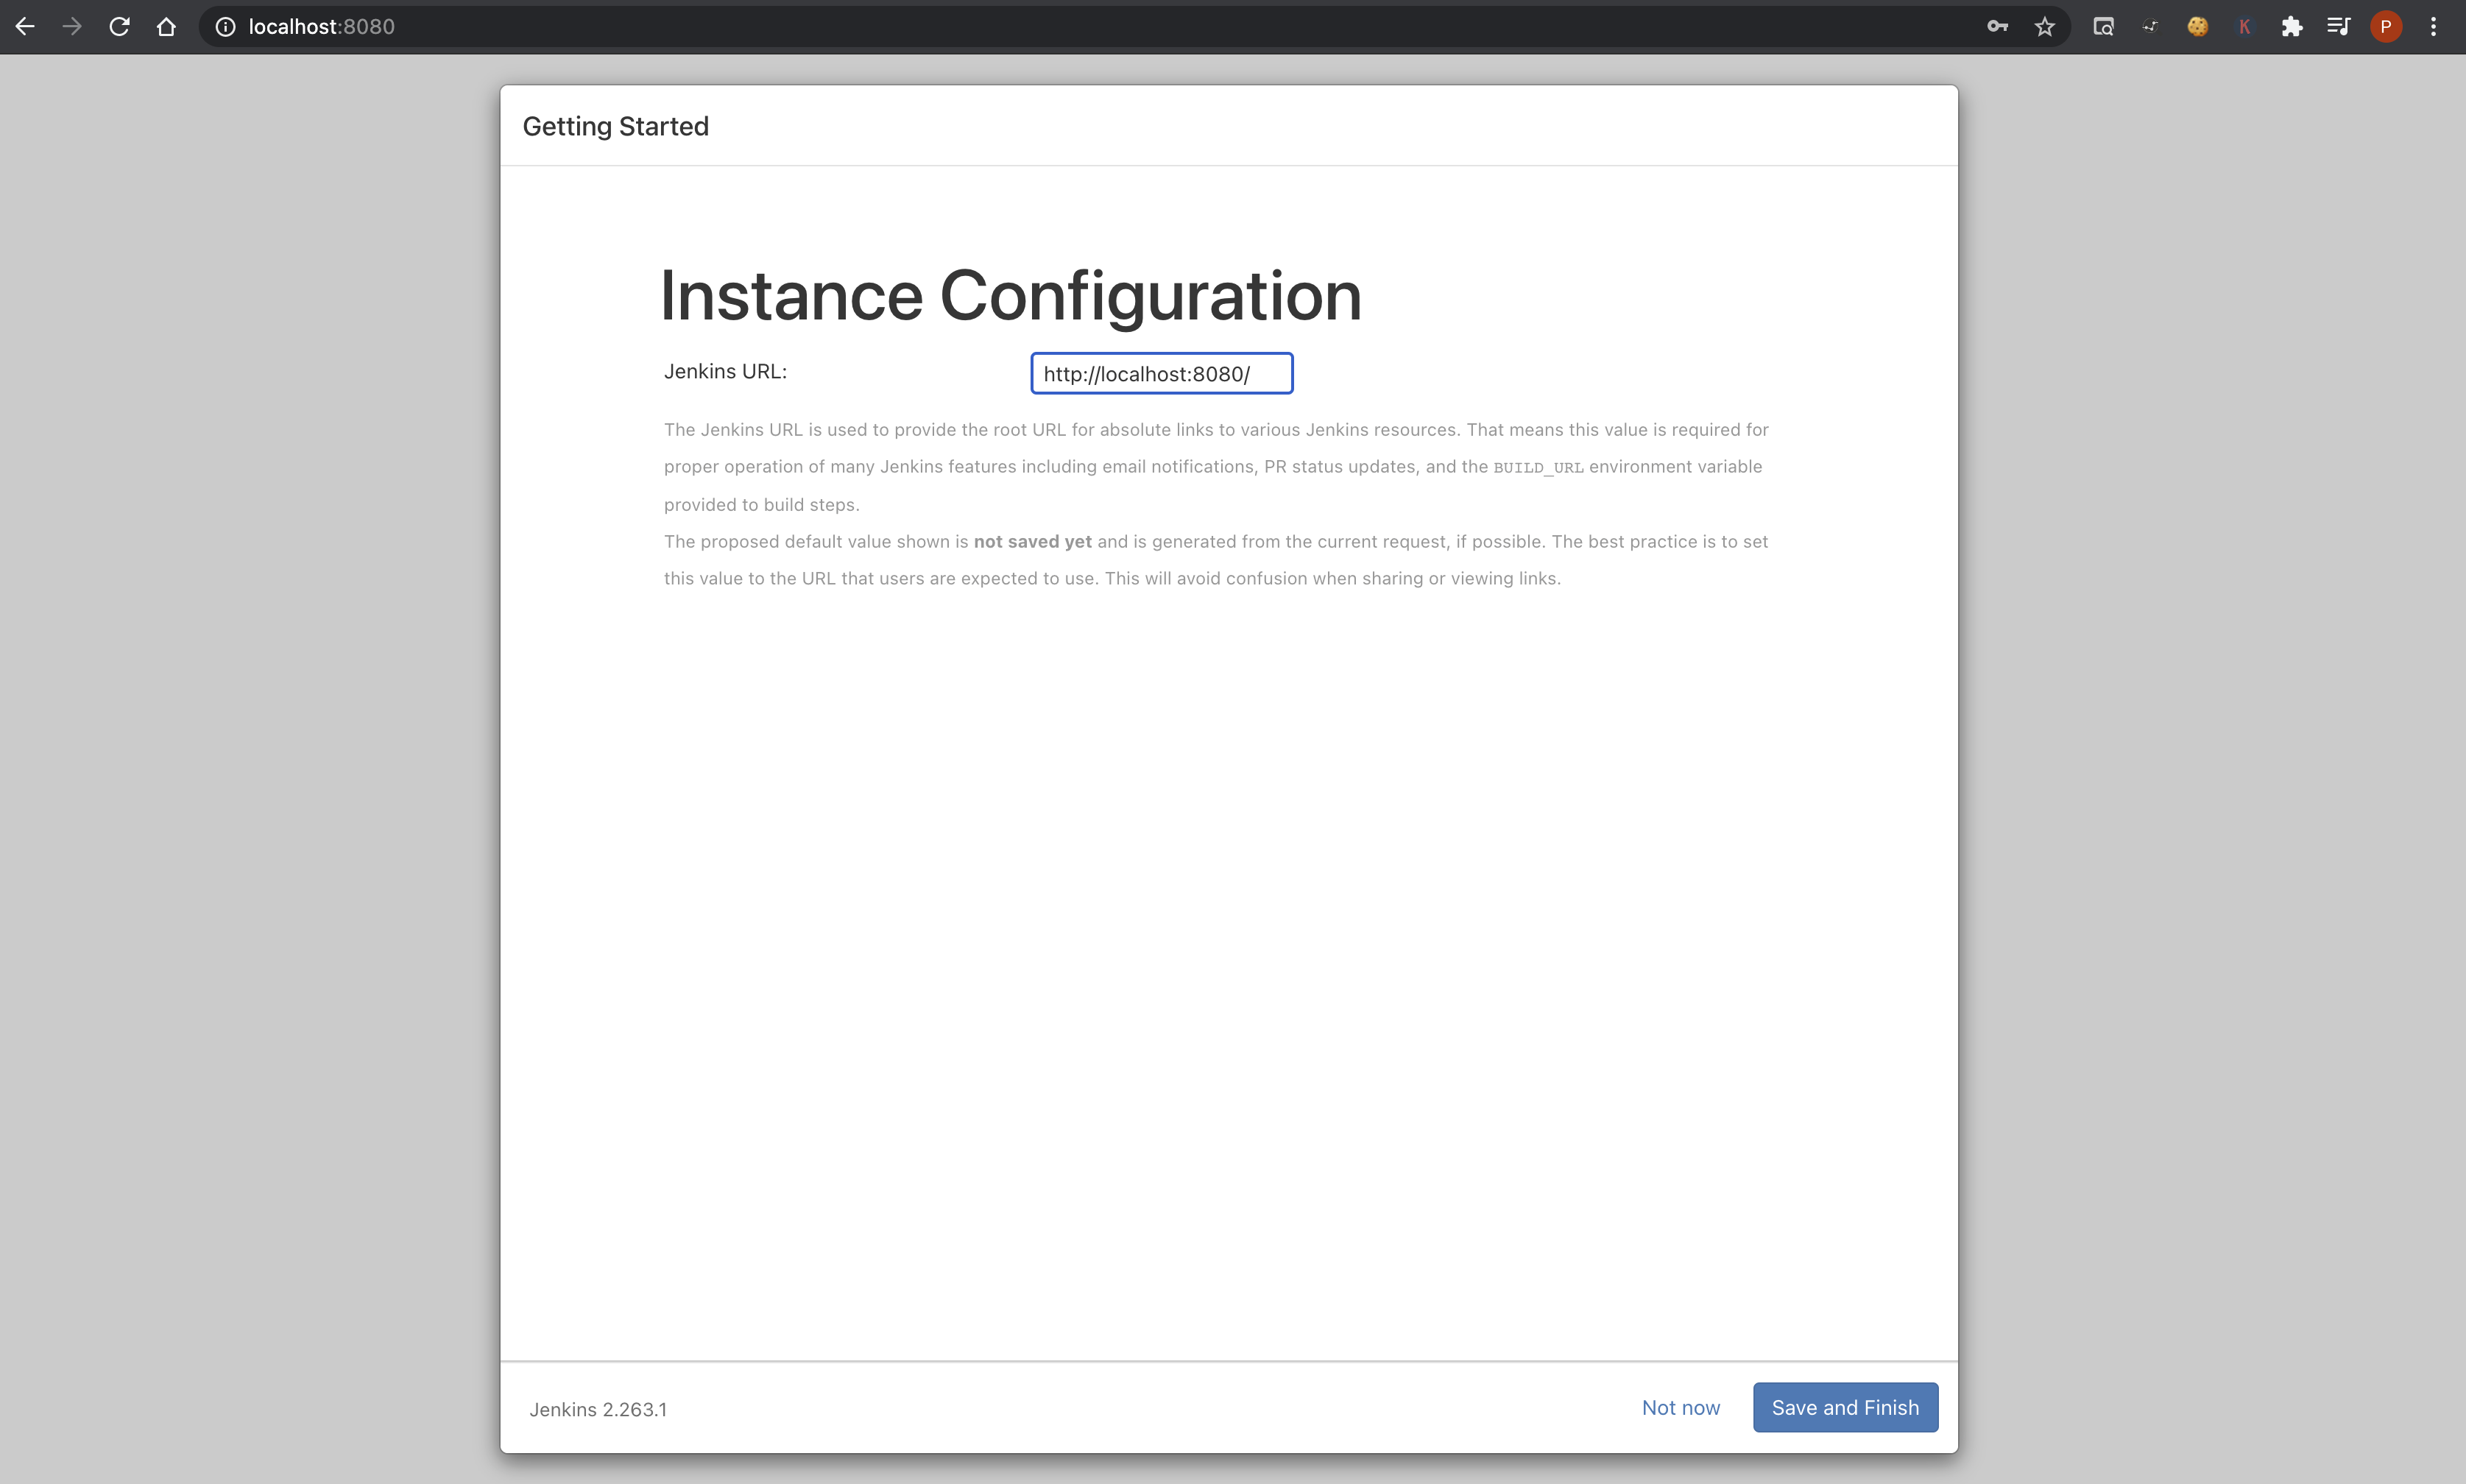
\includegraphics[width=10cm]{iz-Jenkins-port.png}
    \caption{Jenkins port}
    \label{fig:Jenkins-port}
\end{figure}
\begin{figure}[htbp]
    \centering
    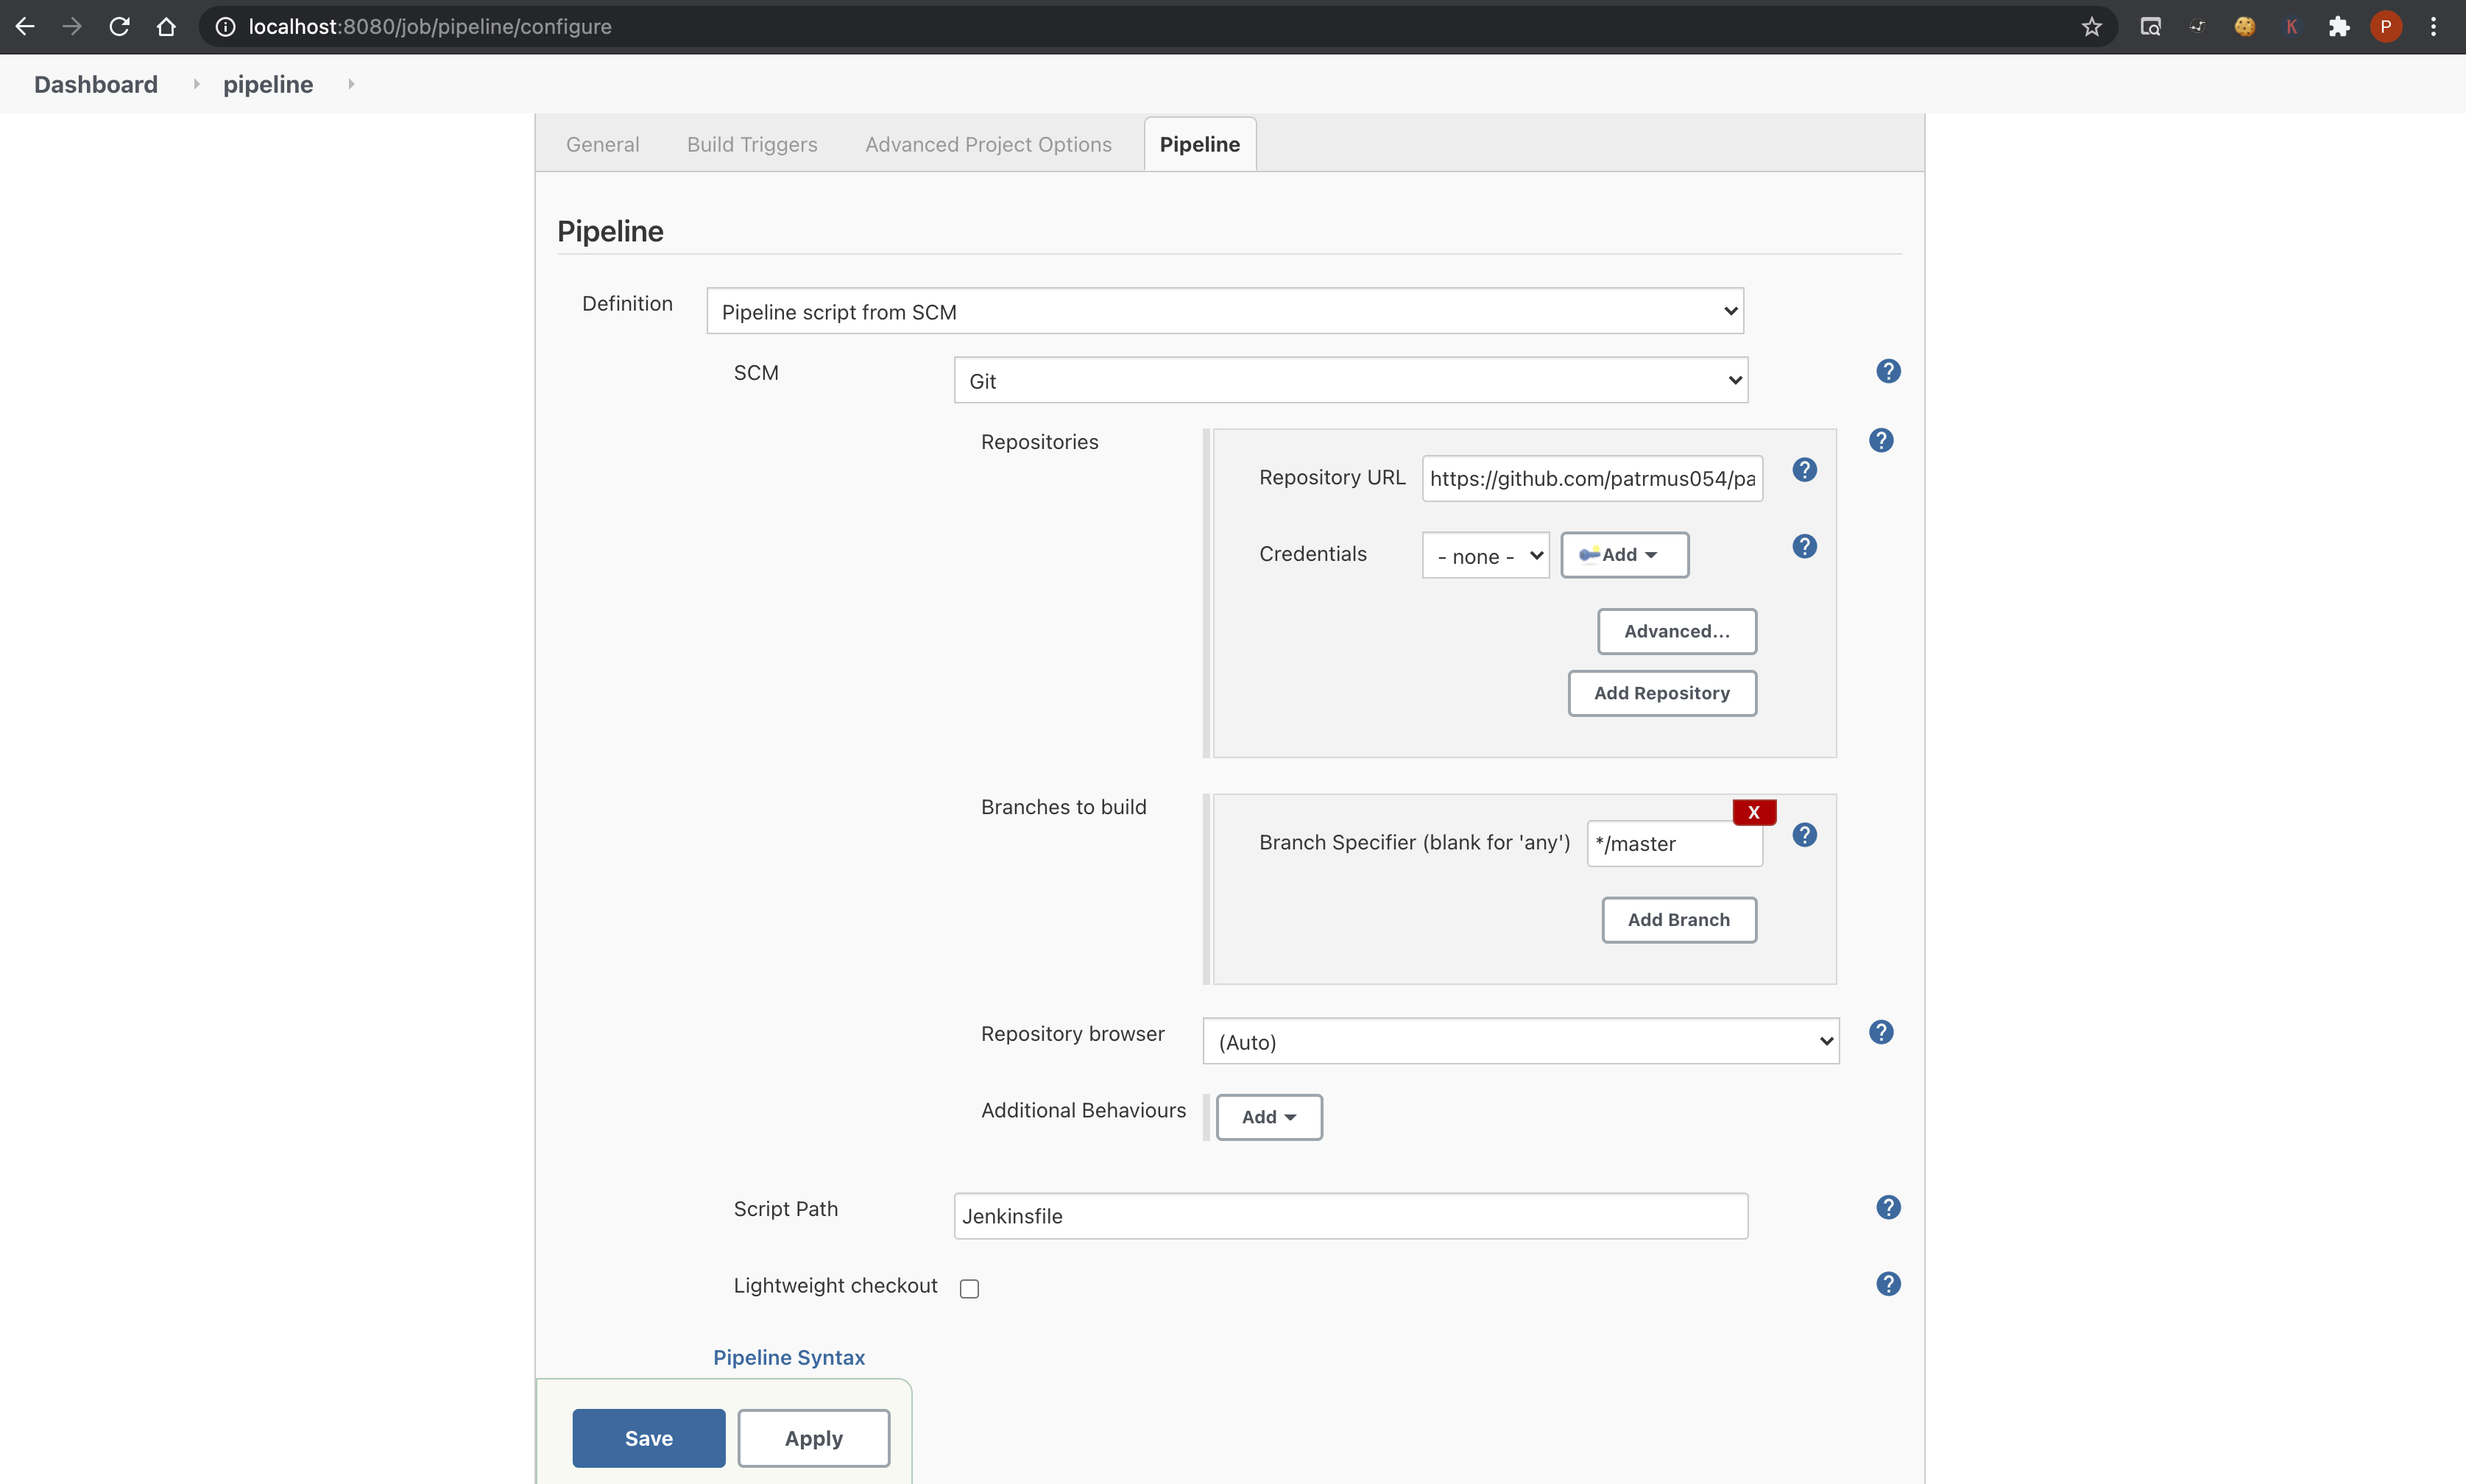
\includegraphics[width=10cm]{iz-pipline.png}
    \caption{pipline}
    \label{fig:pipeline}
\end{figure}


\subsection{Jenkinsfile} 
Jenkinsfile jest plikiem, w którym definiujemy wszystkie kroki, które mają zostać podjęte w ramach Jenkins pipeline. Mamy również możliwość wyboru, które zadania na jakich slave'ach mają zostać wykonane oraz inne metody konfiguracji pipline'u

W naszym projekcie plik ten składa się z czterech następujących kroków:

\begin{lstlisting}
    node {  
        
	    def mvnHome = tool 'maven-3.6.3'
	    def dockerImage
	    def dockerImageTag = "pracainzynierka${env.BUILD_NUMBER}"
		def DOCKER_FILES_DIR = "./initial"
		def dockerfile = "Dockerfile"
	    
	    stage('Clone Repo') { // for display purposes
	      git 'https://github.com/patrmus054/papryk-inzynier.git'           
	      mvnHome = tool 'maven-3.6.3'
	    }    
	  
	    stage('Build Project') {
	      sh "'${mvnHome}/bin/mvn' clean install -f ./initial/pom.xml"
	    }
			
	    stage('Build Docker Image') {
	      dockerImage = docker.build("pracainzynierka:${env.BUILD_NUMBER}", "-f ${DOCKER_FILES_DIR}/${dockerfile} ${DOCKER_FILES_DIR}")
	    }
	   
	    stage('Deploy Docker Image'){
	      echo "Docker Image Tag Name: ${dockerImageTag}"
		  sh "docker run pracainzynierka:${env.BUILD_NUMBER} -p 2222:2222 "
	    }
}
\end{lstlisting}

Na początku pliku definiujemy zmienne lokalne, potem w kolejnych krokach zasadniczo wszystkie kroki, które musieliśmy wcześniej wpisywać "ręcznie": pobranie projektu z repozytorium, budowanie aplikacji, budowanie obrazu Dockera i uruchamianie aplikacji. 

\subsection{Podsumowanie projektu}

W dzisiejszym środowisku IT mamy mnogość narzędzi które pozwalają w stosunkowo prosty sposób automatyzować procesy związane z inżynierią oprogramowania i nie tylko. Jenkins jest w branży od pewnego czasu i dzięki rozbudowanemu ekosystemowi mamy możliwość automatyzować rzeczy, które wcześniej zajmowały dużo czasu. W projekcie wykorzystaliśmy możliwości narzędzia do stworzenia dwóch działających kontenerów. Rozwiązanie ma jednak jedynie charakter prezentacyjny i nie powinno stanowić inspiracji do produkcji przemysłowej. 
